\section{Dummy signal testing of the regular and variational Autoencoder}

Another important part of benchmarking the algorithm is to test it on a signal sample. This is the closest test we can do before
we no longer can alter the algorithm, as that would be supervised learning. Results from both the regular and the variational autoencoder 
are shown below. 

\subsection*{Autoencoder}

\begin{figure}[h!]
    \centering
    \begin{subfigure}{.45\textwidth}
        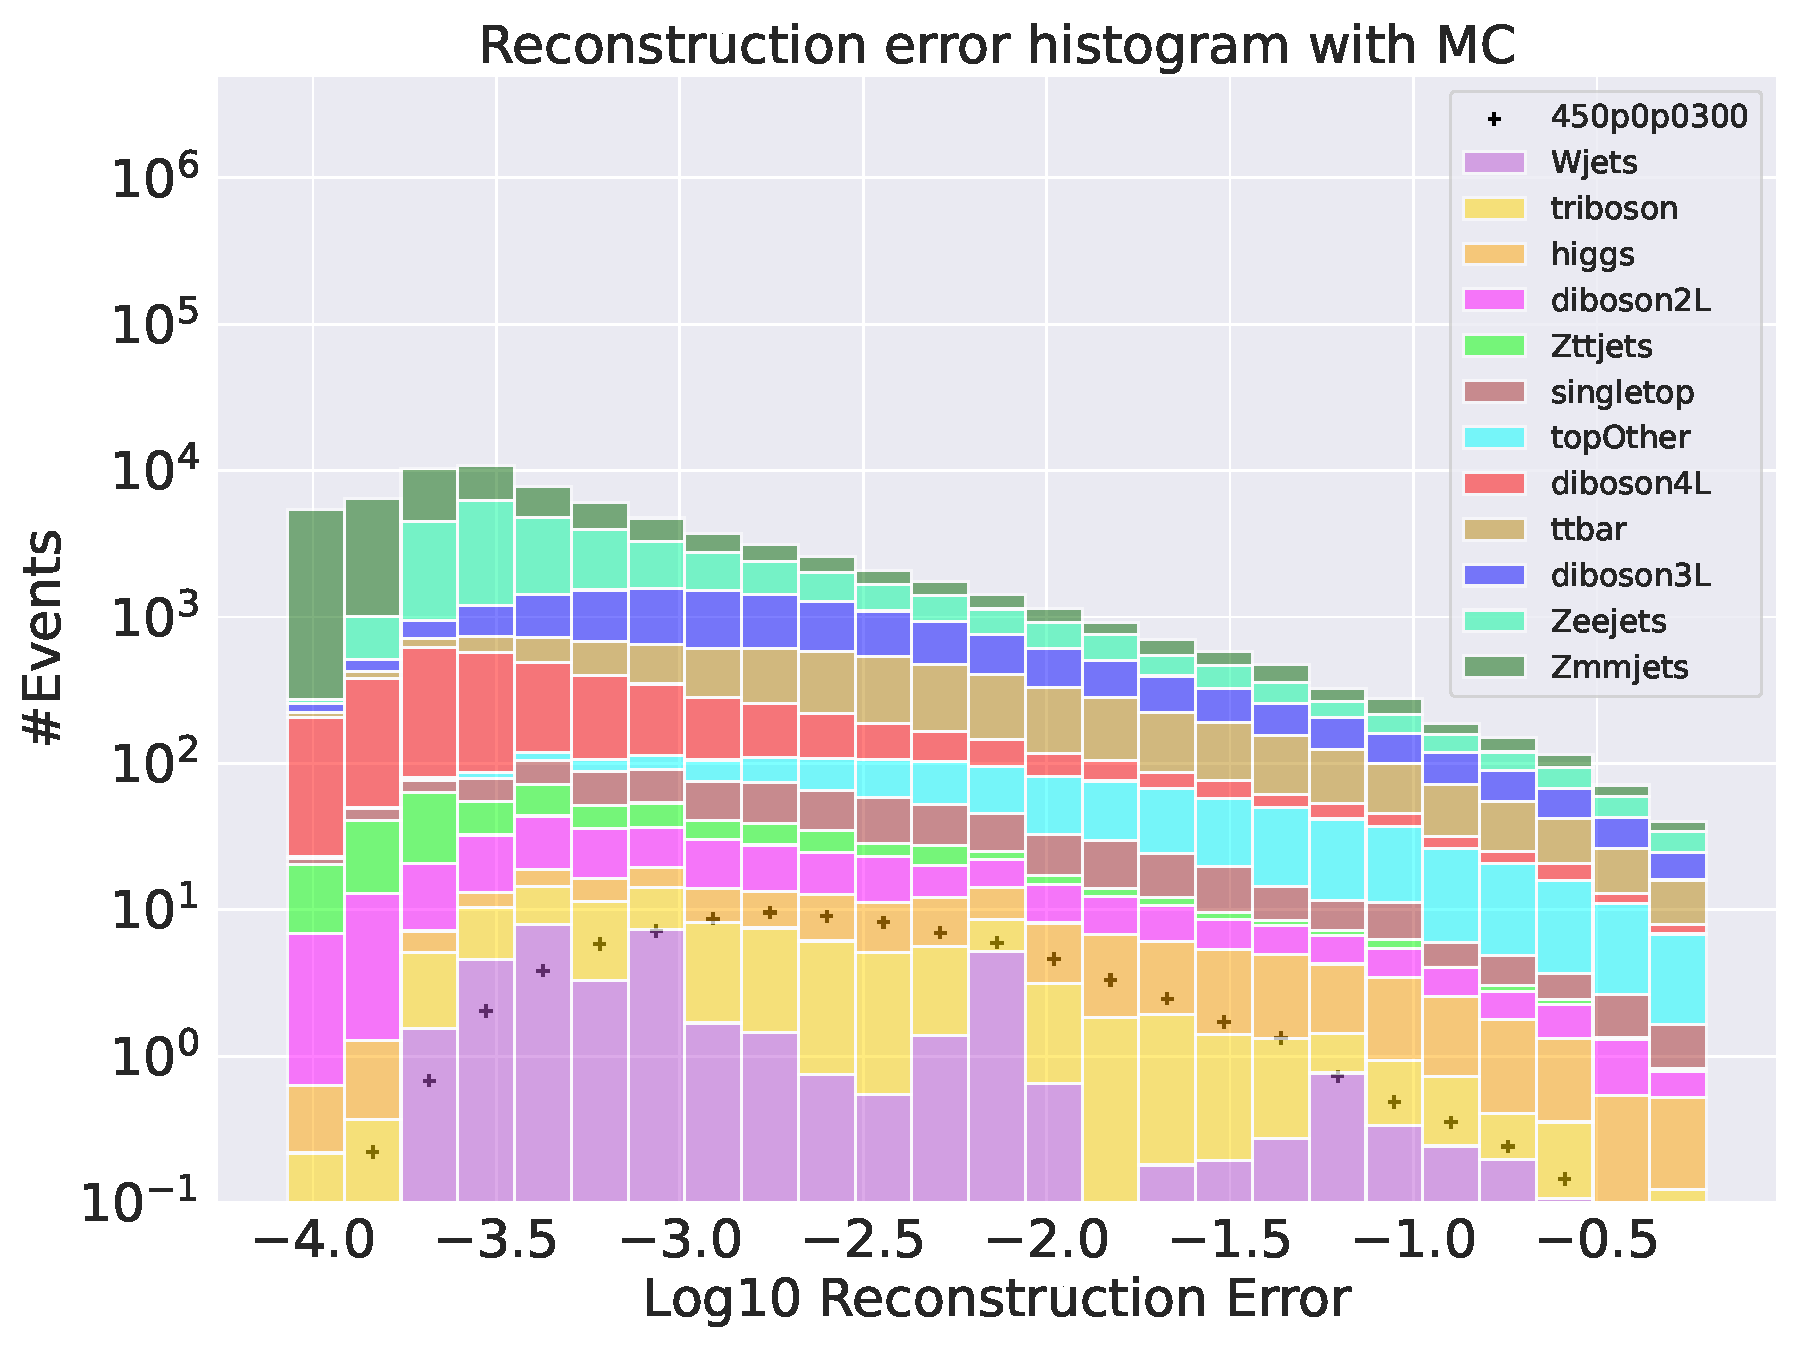
\includegraphics[width=\textwidth]{Figures/AE_testing/small/b_data_recon_big_rm3_feats_sig_450p0p0300.pdf}
        \caption{Reconstruction error on validation SM MC from the Autoencoder. The susy signal is the $450-300$ sample. 
        No significant separation of the distributions are found. }
        \label{fig:ae_susy_450_300_recon}
    \end{subfigure}
    \hfill
    \begin{subfigure}{.45\textwidth}
        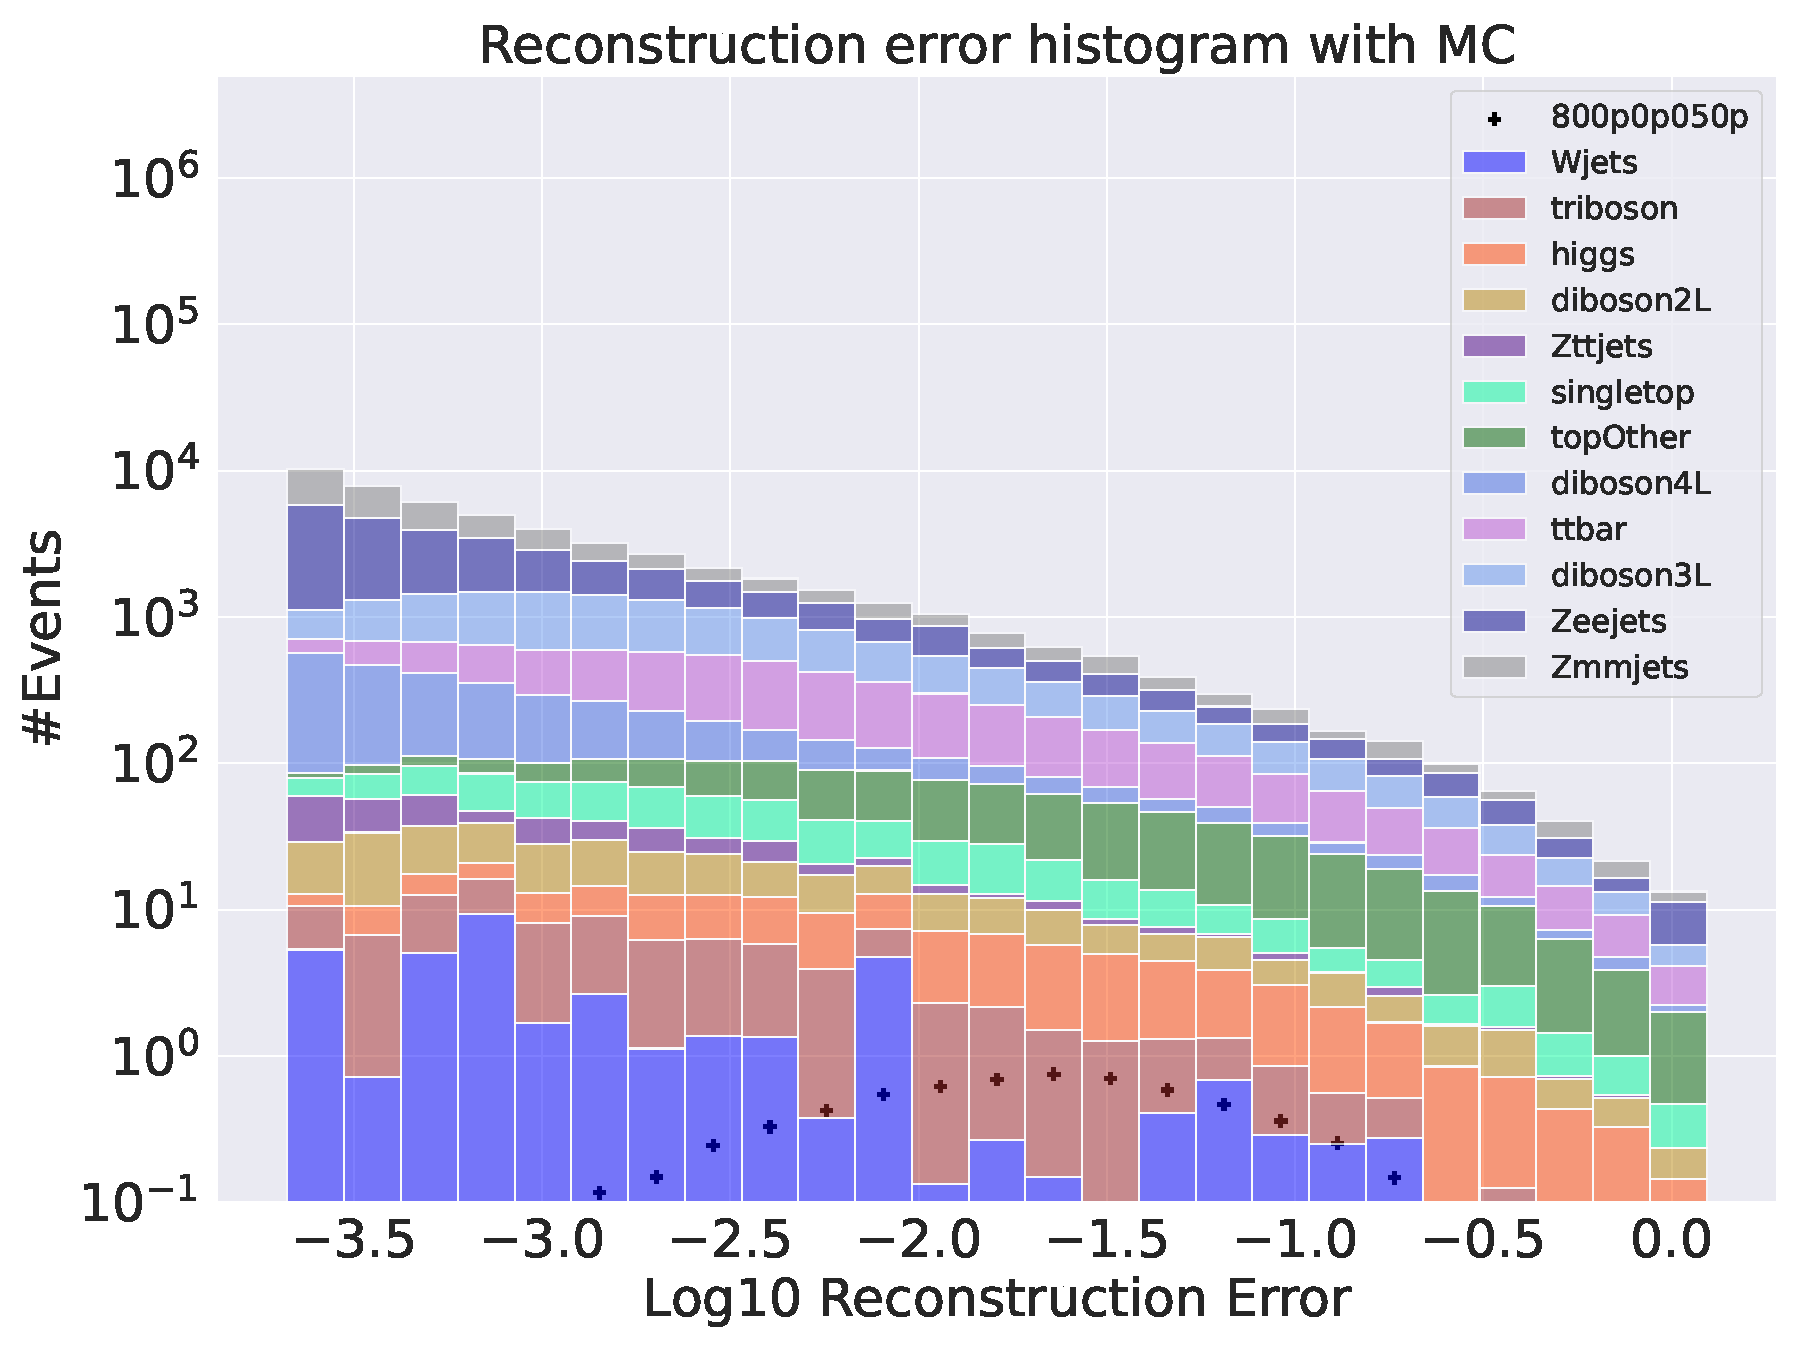
\includegraphics[width=\textwidth]{Figures/AE_testing/small/b_data_recon_big_rm3_feats_sig_800p0p050p.pdf}
        \caption{Reconstruction error on validation SM MC from the Autoencoder. The susy signal is the $800-50$ sample. 
        No significant separation of the distributions are found. }
        \label{fig:ae_susy_800_50_recon}
    \end{subfigure}
    \hfill
    \begin{subfigure}{.45\textwidth}
        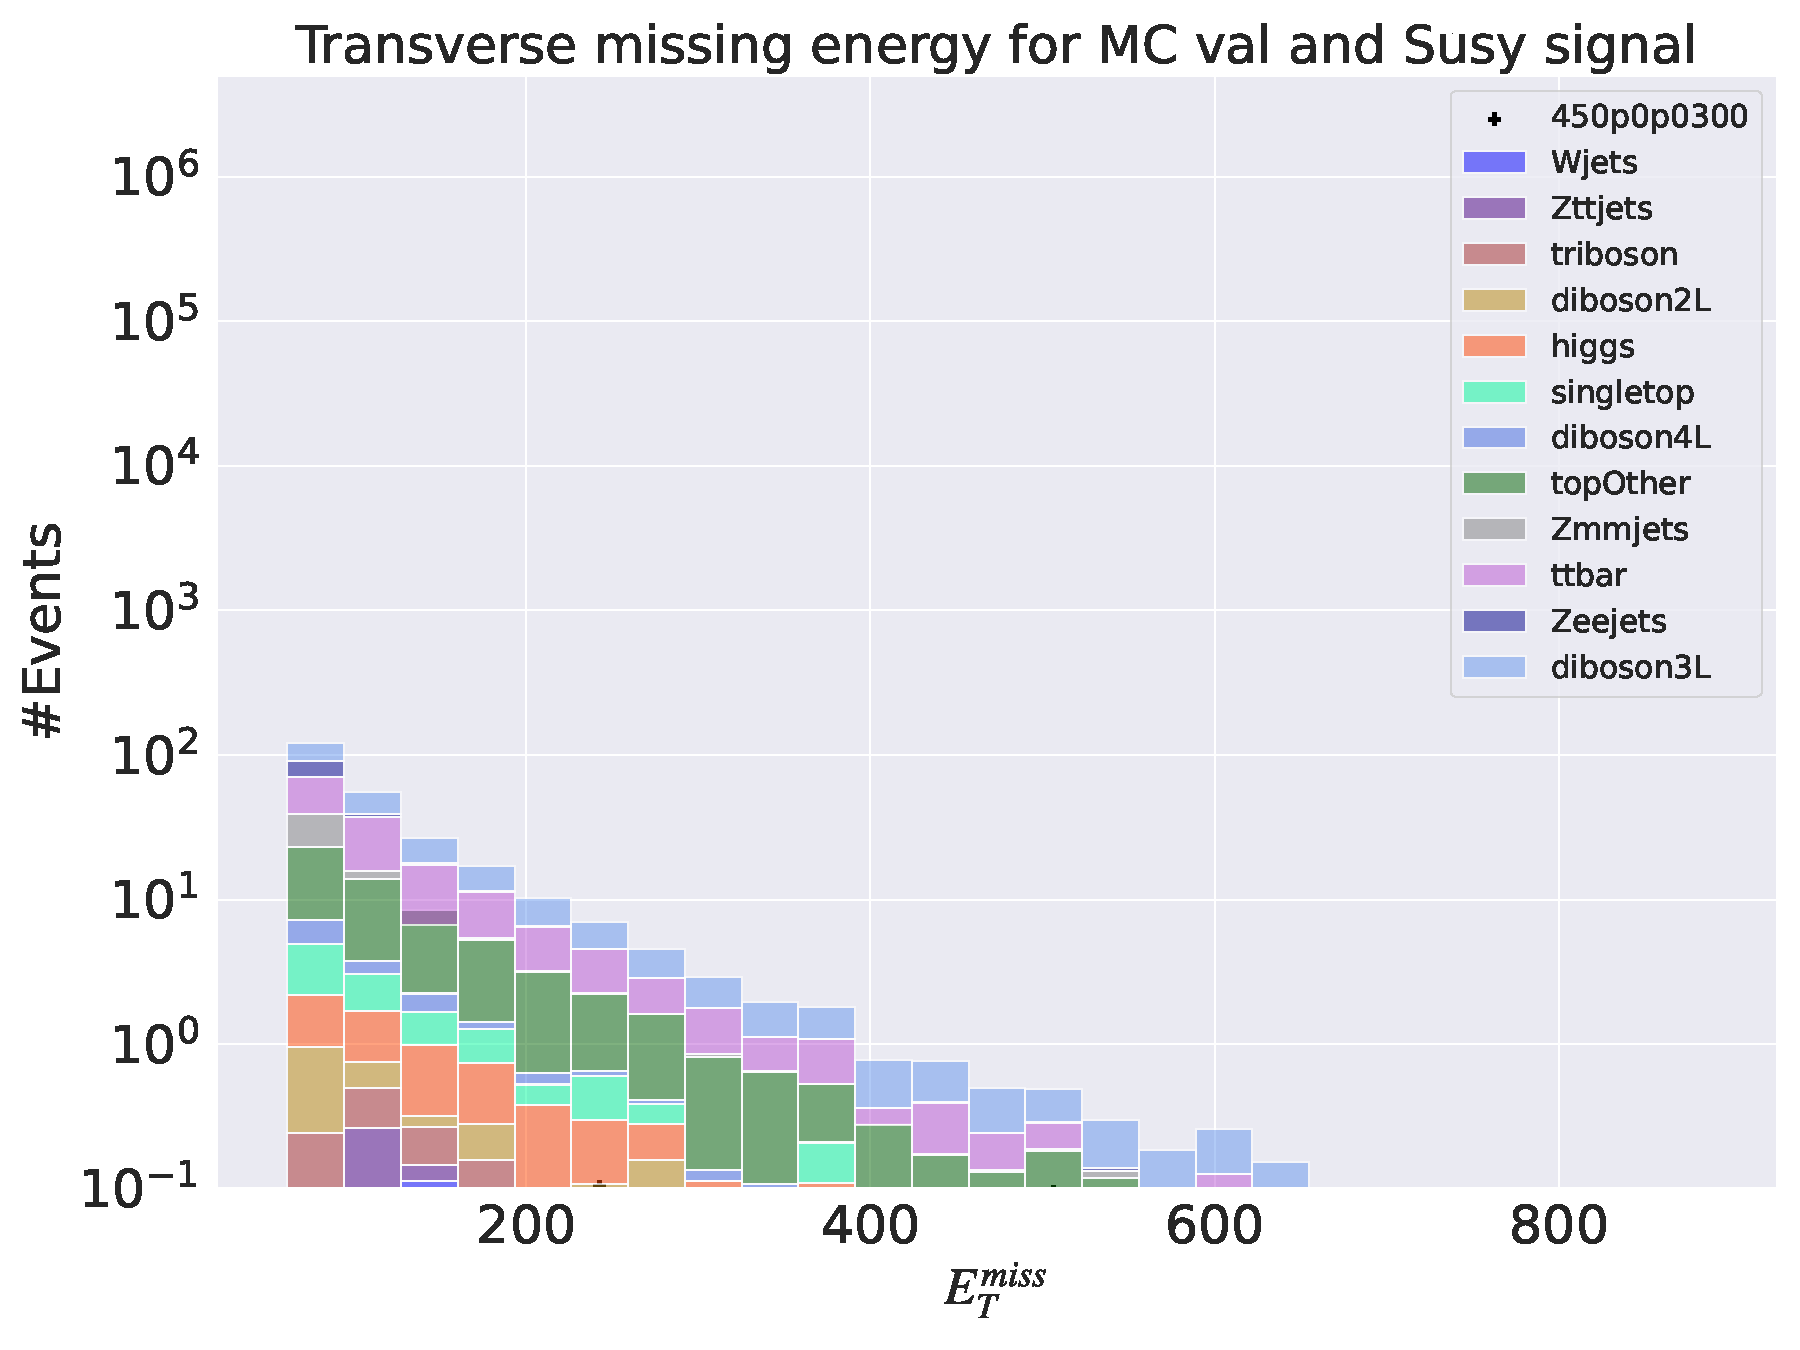
\includegraphics[width=\textwidth]{Figures/AE_testing/small/b_data_recon_big_rm3_feats_sig_450p0p0300_etmiss.pdf}
        \caption{Etmiss bump search for the $450-300$ susy signal. Here events are selected only if reconstruction error is larger than 1. No significant 
        separation of distribution found.}
        \label{fig:ae_susy_450_300_trilep}
    \end{subfigure}
    \hfill        
    \begin{subfigure}{.45\textwidth}
        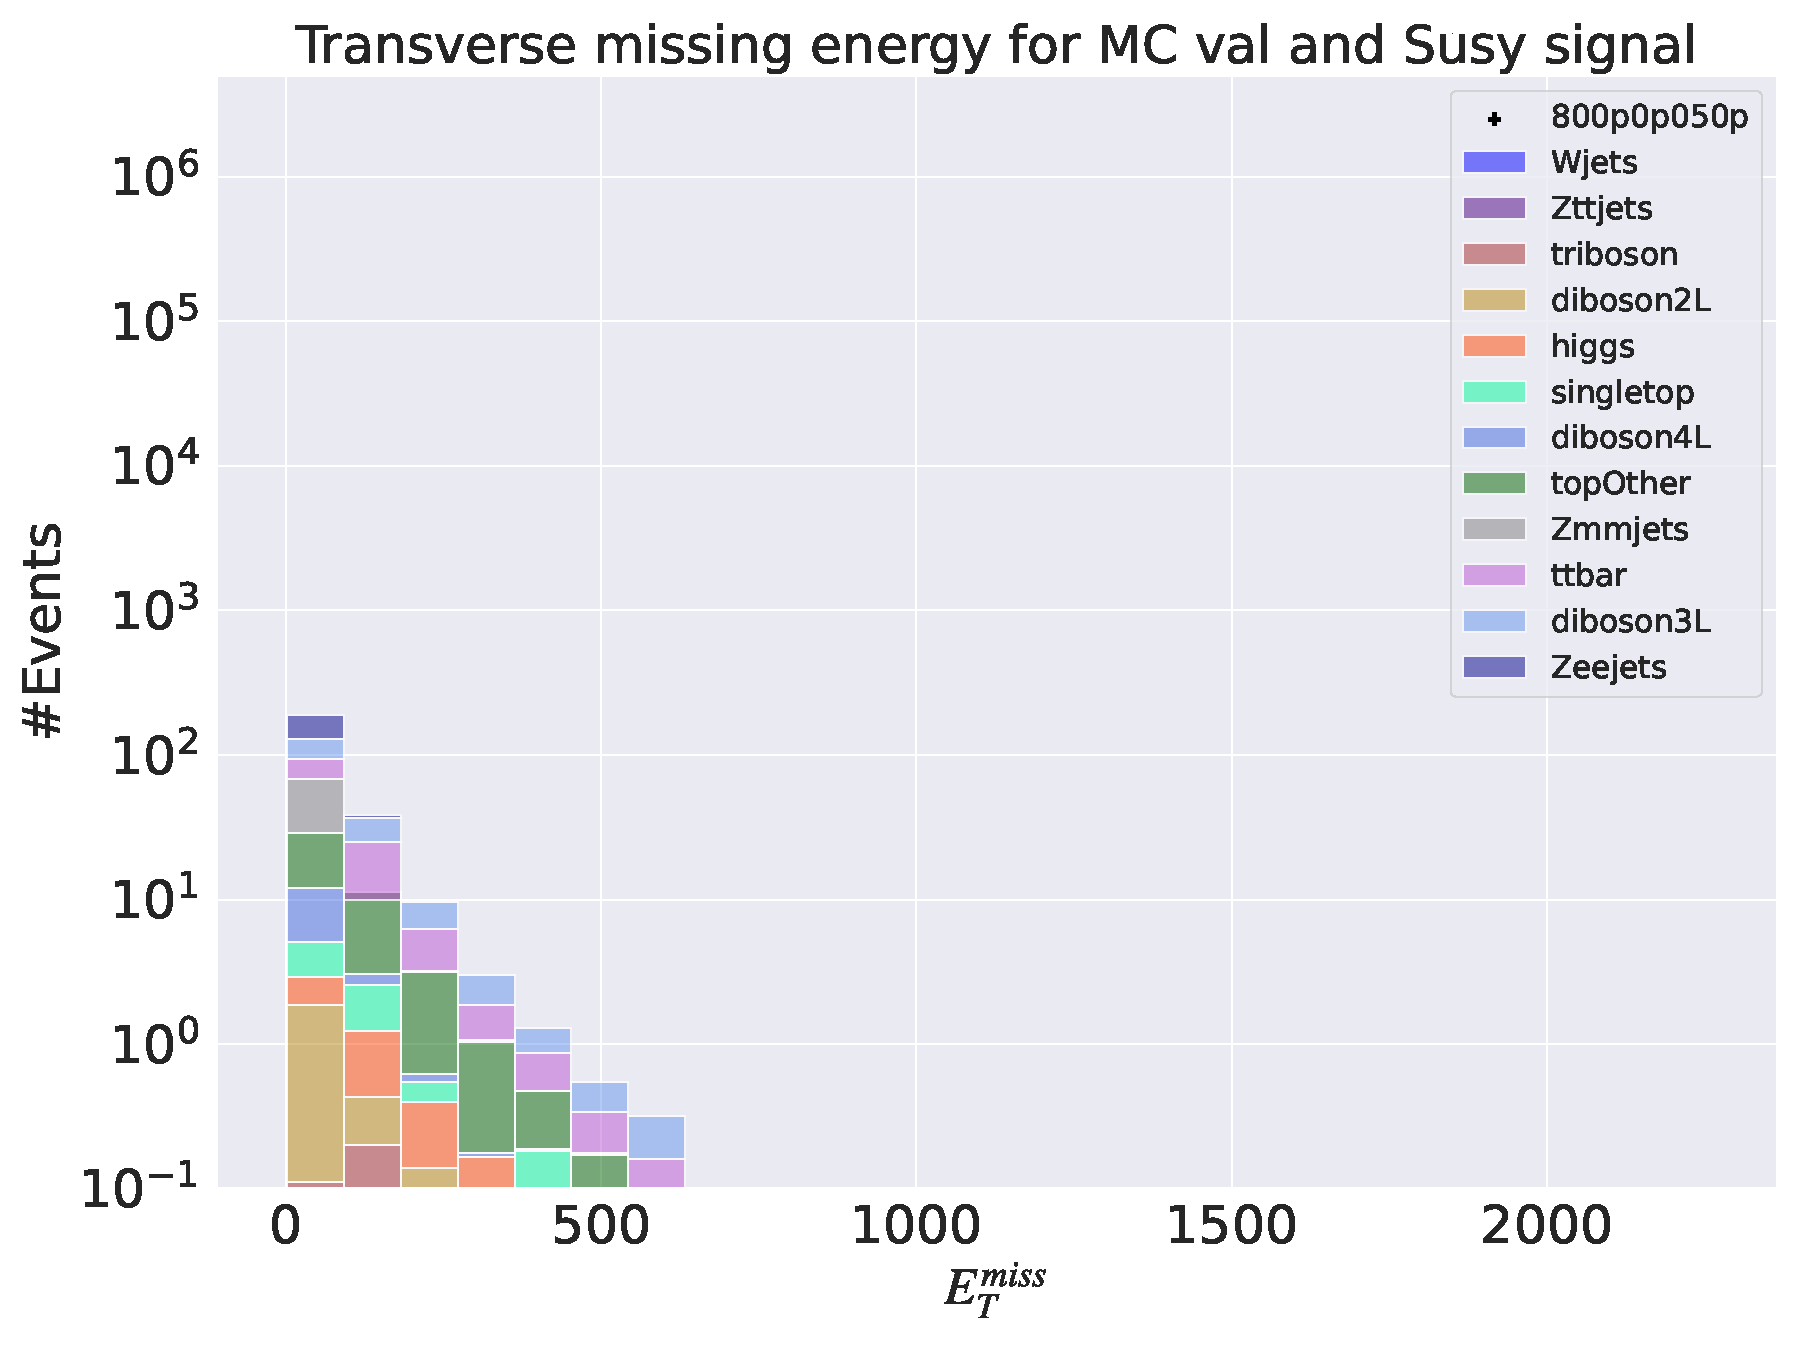
\includegraphics[width=\textwidth]{Figures/AE_testing/small/b_data_recon_big_rm3_feats_sig_800p0p050p_etmiss.pdf}
        \caption{etmiss bump search for the $800-50$ susy signal. Here events are selected only if reconstruction error is larger than 1. No significant 
        separation of distribution found.}
        \label{fig:ae_susy_800_50_trilep}
    \end{subfigure} 
    \hfill     
    \caption{Etmiss bump search on the $450-300$ and $800-50$ susy signals. The reconstruction error cut is set to 1.}
    \label{fig:ae_susy_450_300_800_50_recon_trilep}
\end{figure}


\subsection*{Variational Autoencoder}

\begin{figure}[h!]
    \centering
    \begin{subfigure}{.45\textwidth}
        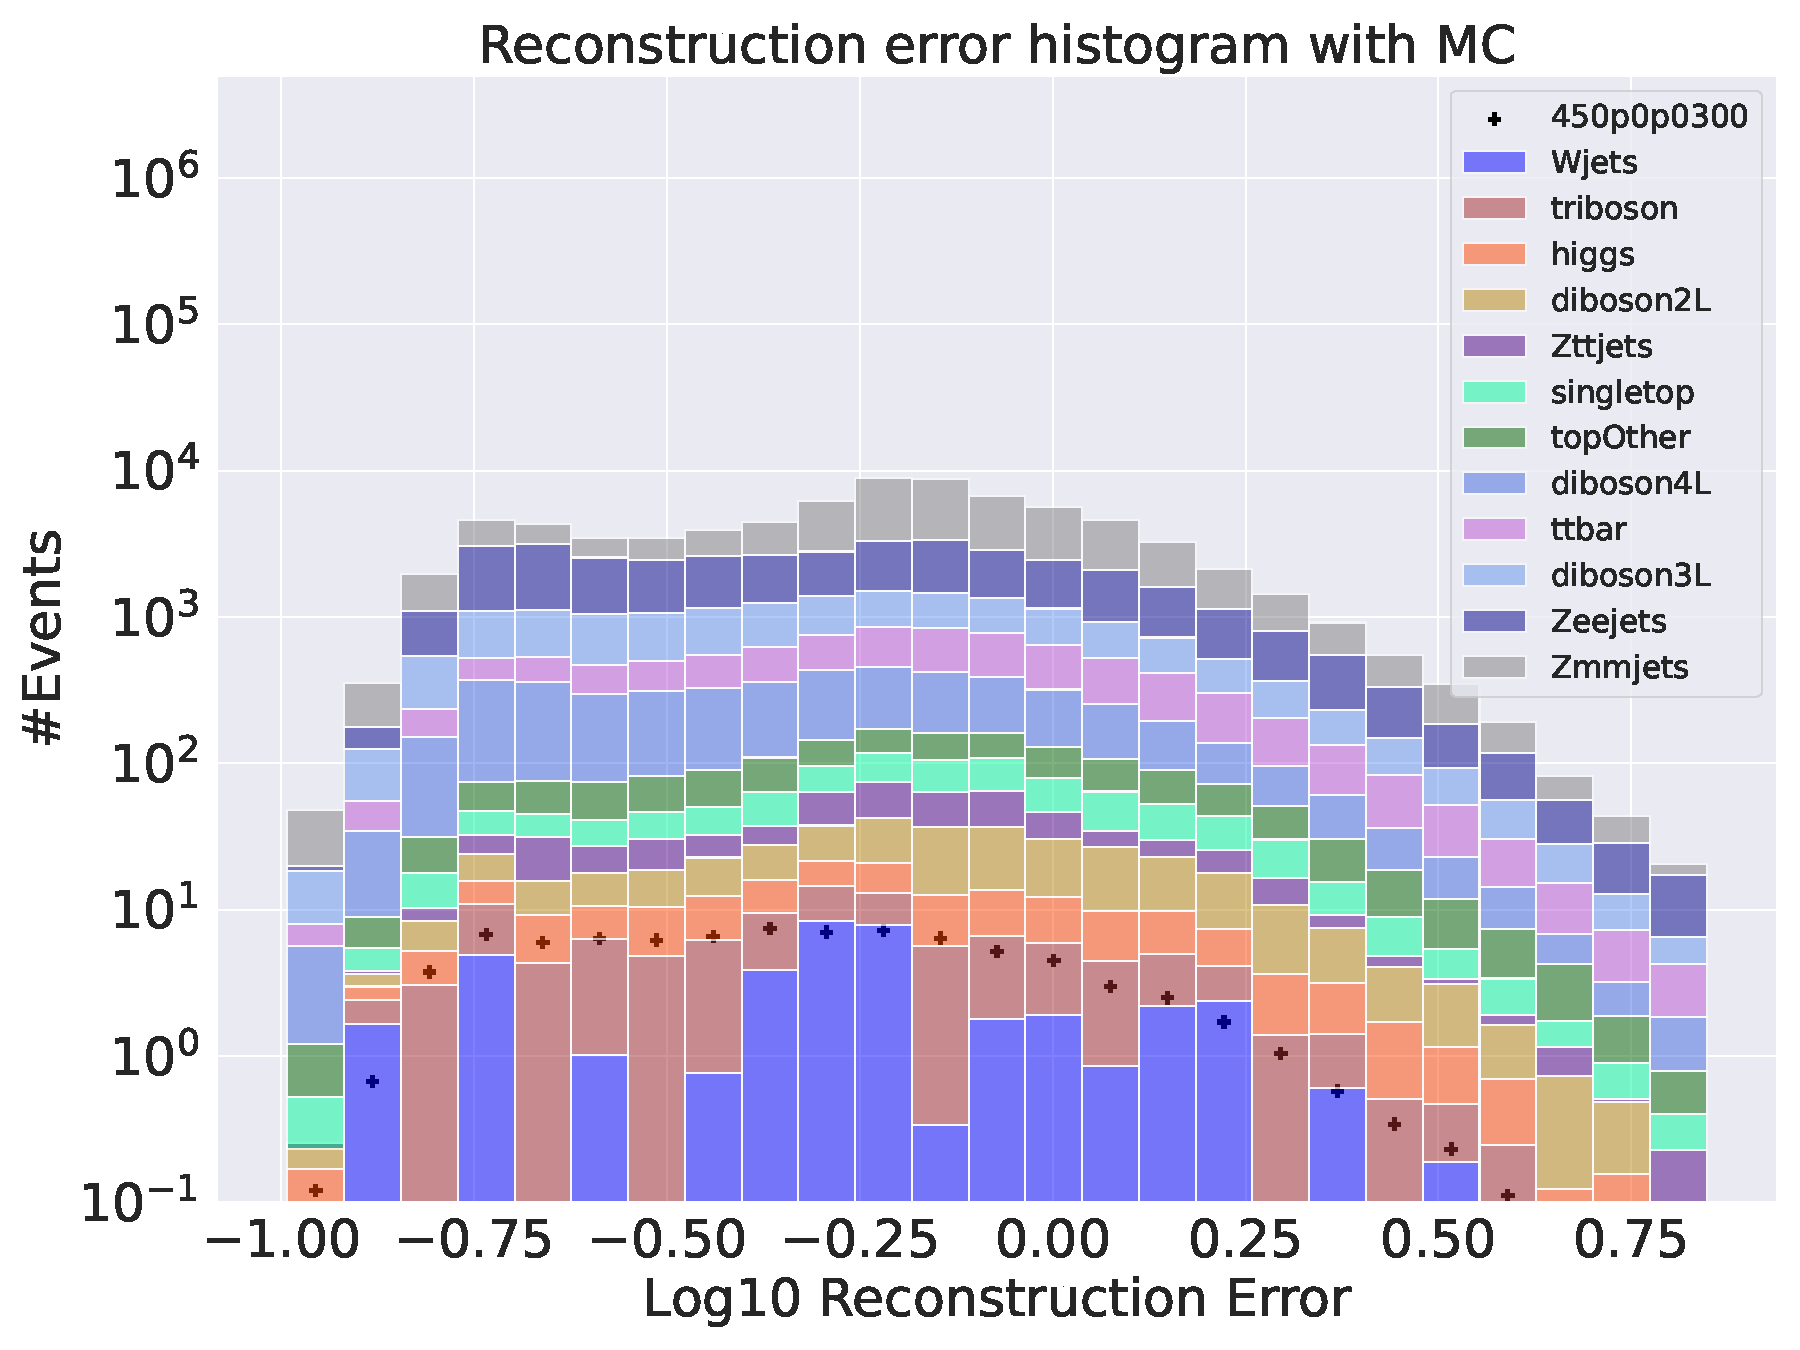
\includegraphics[width=\textwidth]{Figures/VAE_testing/small/b_data_recon_big_rm3_feats_sig_450p0p0300.pdf}
        \caption{Reconstruction error on validation SM MC from the variational Autoencoder. The susy signal is the $450-300$ sample. 
        No significant separation of the distributions are found. }
        \label{fig:vae_susy_450_300_recon}
    \end{subfigure}
    \hfill
    \begin{subfigure}{.45\textwidth}
        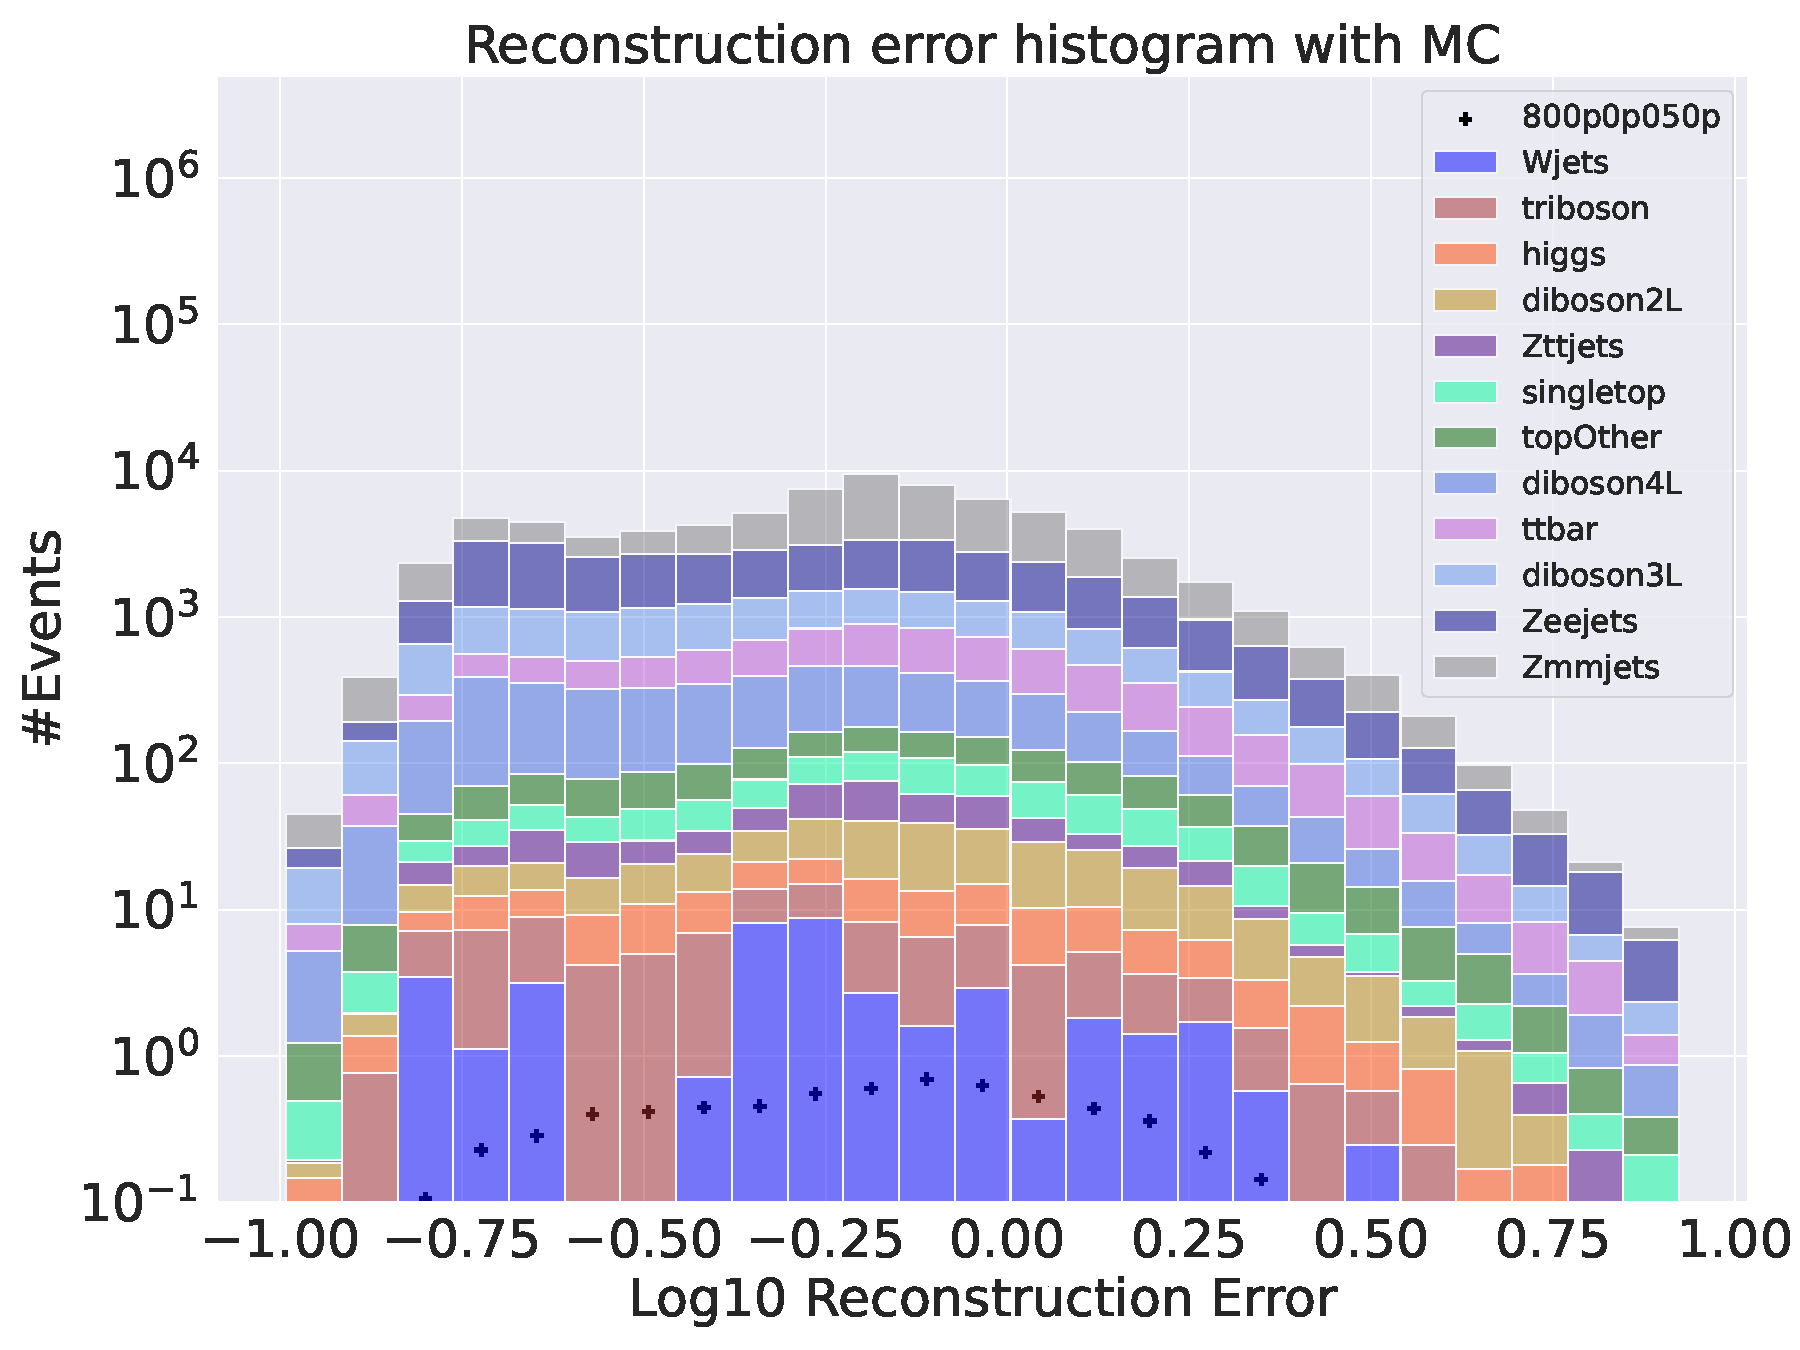
\includegraphics[width=\textwidth]{Figures/VAE_testing/small/b_data_recon_big_rm3_feats_sig_800p0p050p.pdf}
        \caption{Reconstruction error on validation SM MC from the variational Autoencoder. The susy signal is the $800-50$ sample. 
        No significant separation of the distributions are found. }
        \label{fig:vae_susy_800_50_recon}
    \end{subfigure}
    \hfill
    \begin{subfigure}{.45\textwidth}
        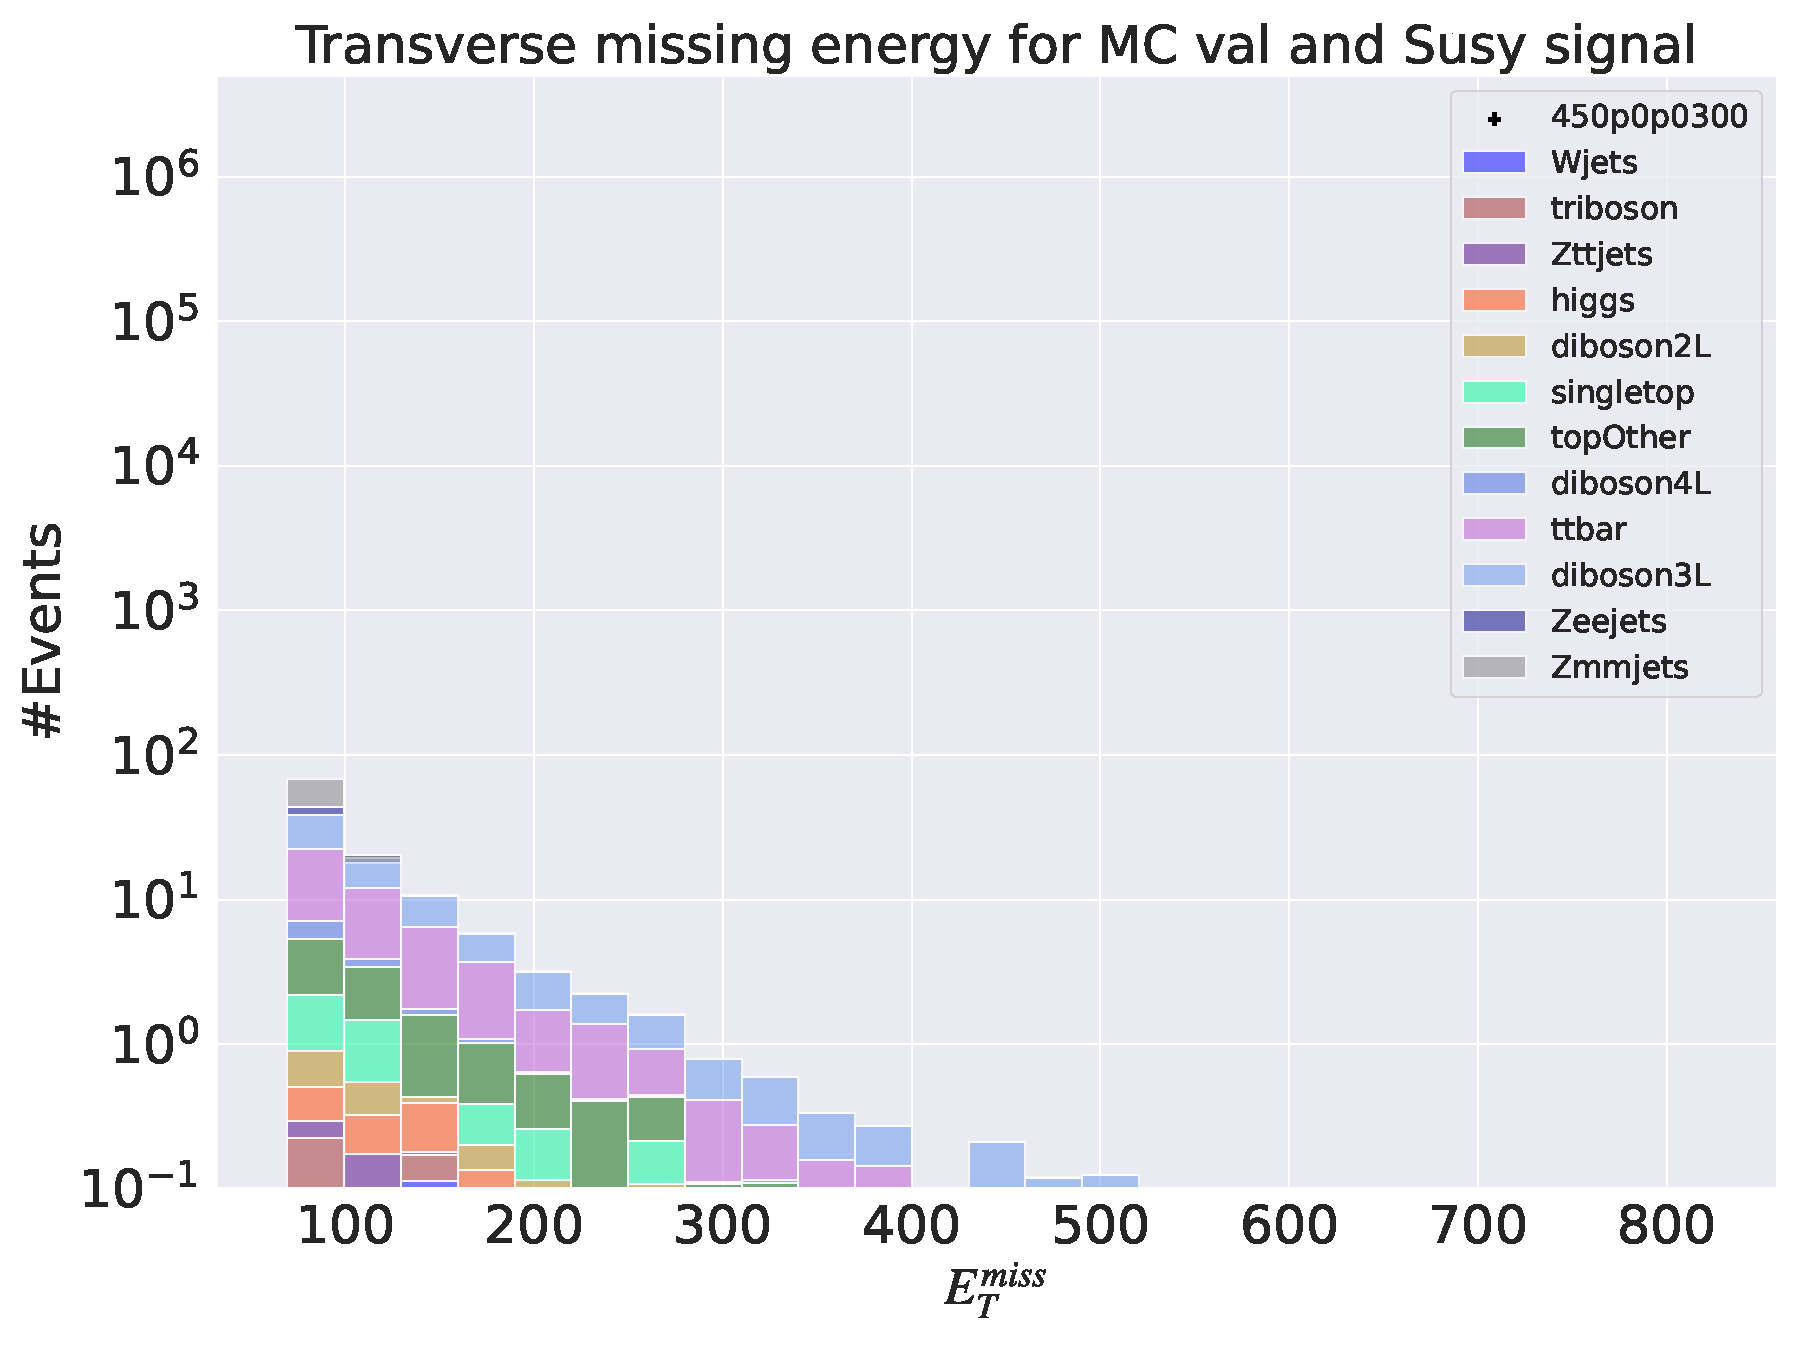
\includegraphics[width=\textwidth]{Figures/VAE_testing/small/b_data_recon_big_rm3_feats_sig_450p0p0300_etmiss.pdf}
        \caption{etmiss bump search for the $450-300$ susy signal. Here events are selected only if reconstruction error is larger than 1. No significant 
        separation of distribution found.}
        \label{fig:vae_susy_450_300_trilep}
    \end{subfigure}
    \hfill   
    \begin{subfigure}{.45\textwidth}
        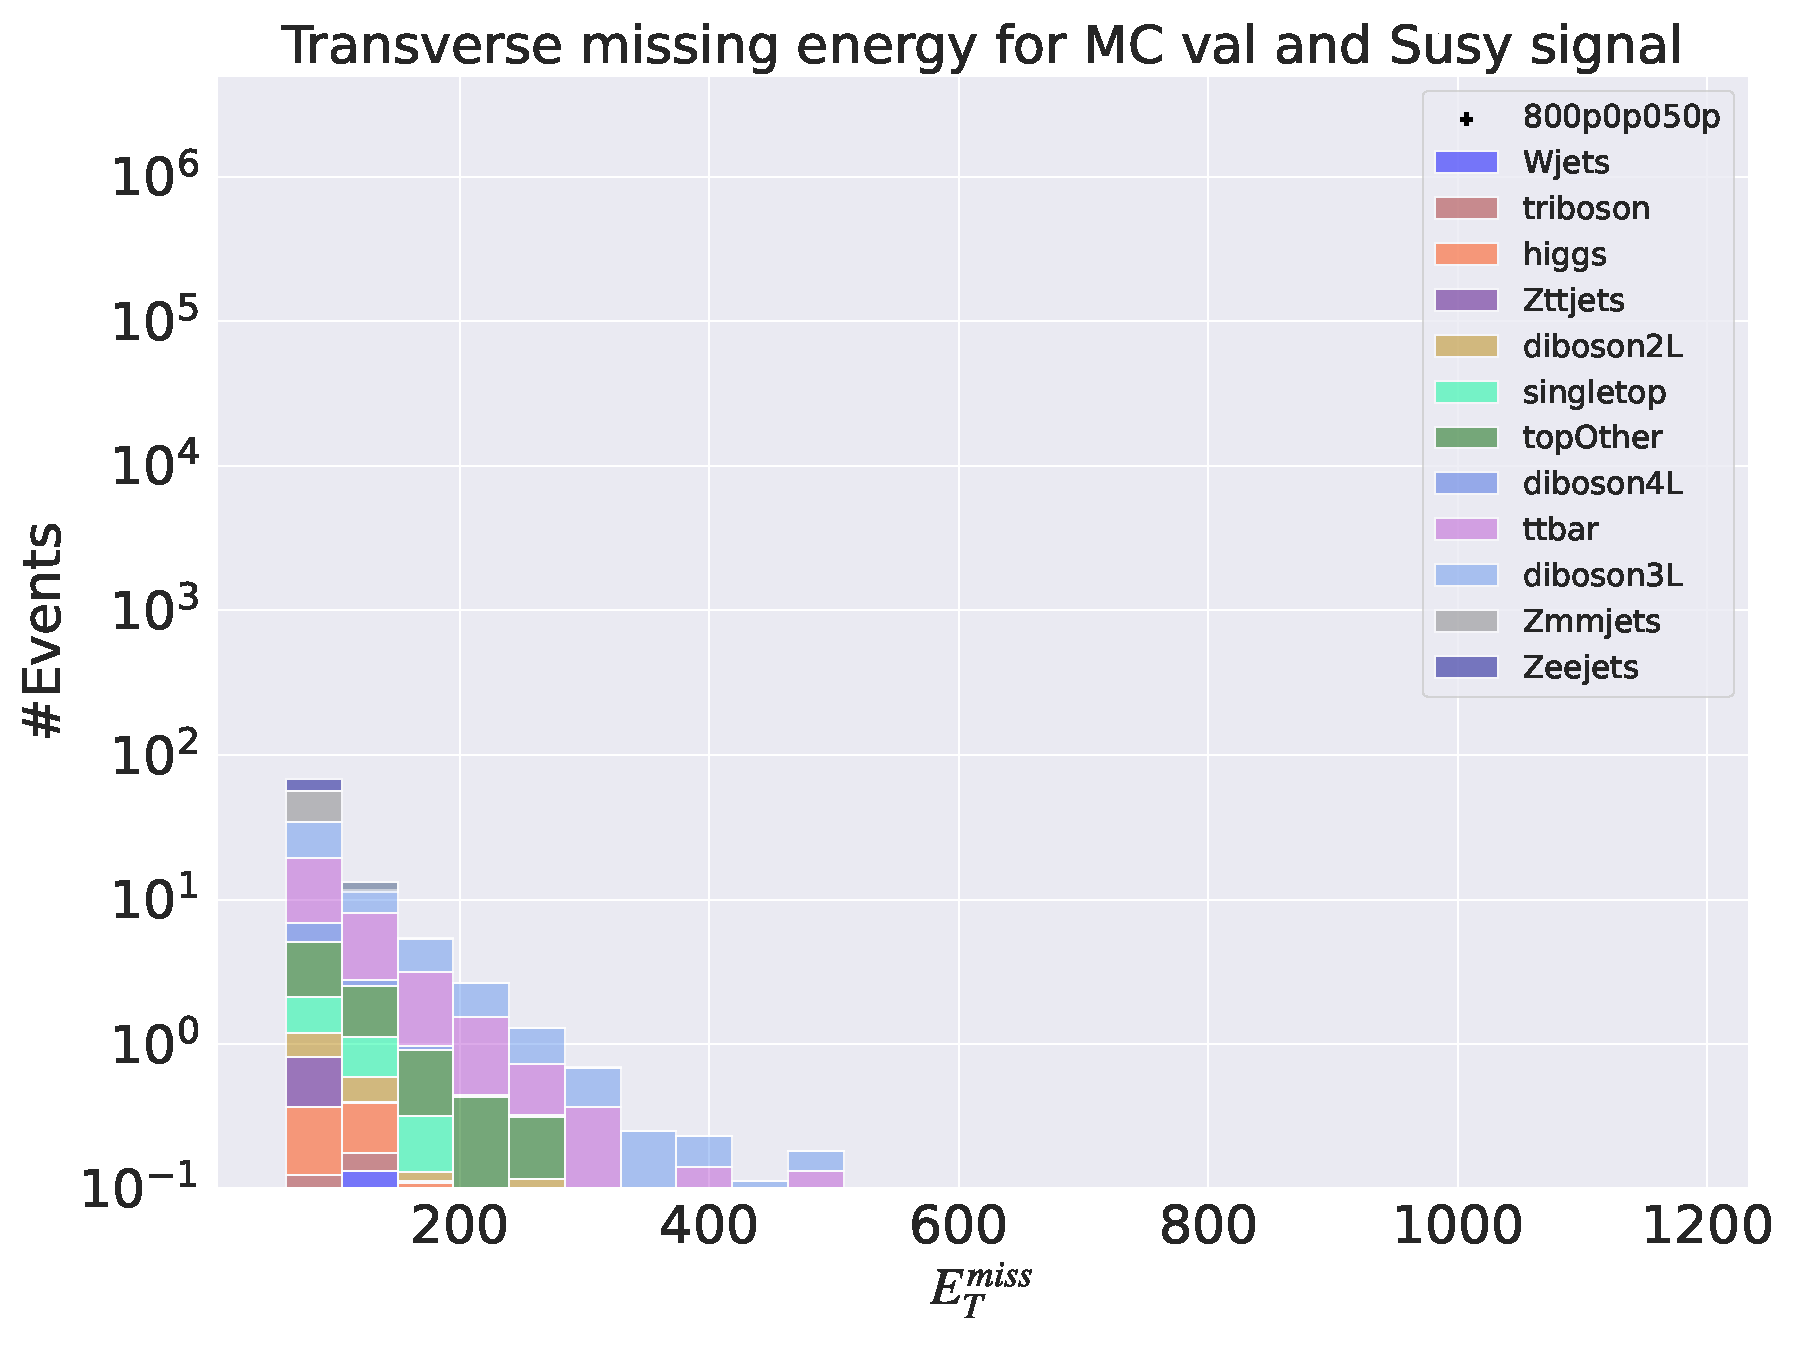
\includegraphics[width=\textwidth]{Figures/VAE_testing/small/b_data_recon_big_rm3_feats_sig_800p0p050p_etmiss.pdf}
        \caption{etmiss bump search for the $800-50$ susy signal. Here events are selected only if reconstruction error is larger than 1. No significant 
        separation of distribution found.}
        \label{fig:vae_susy_800_50_trilep}
    \end{subfigure}
    \hfill      
    \caption{ Reconstruction error and etmiss bump search on the $450-300$ and $800-50$ susy signals. The reconstruction error cut is set to 1.}
    \label{fig:vae_susy_450_300_800_50_recon_trilep}
\end{figure}


\newpage
\subsection*{ROC curves on $e_T^{miss}$ and reconstruction error}
Now based on the reconstruction error on the SUSY signals, especially the one in figure \ref{fig:ae_susy_800_50_recon}, it is tempting to declare that the autoencoder 
has done a good job reconstructing the standard model and a poor job on the SUSY signal, resulting in a separation of distributions. However, there is one thing we need to remember. 
The SUSY signals have very high $e_T^{miss}$, so much so that one can separate them by eye on that distribution alone. This is presented in the figure below:

\begin{figure}[h!]
    \centering
    \begin{subfigure}{.45\textwidth}
    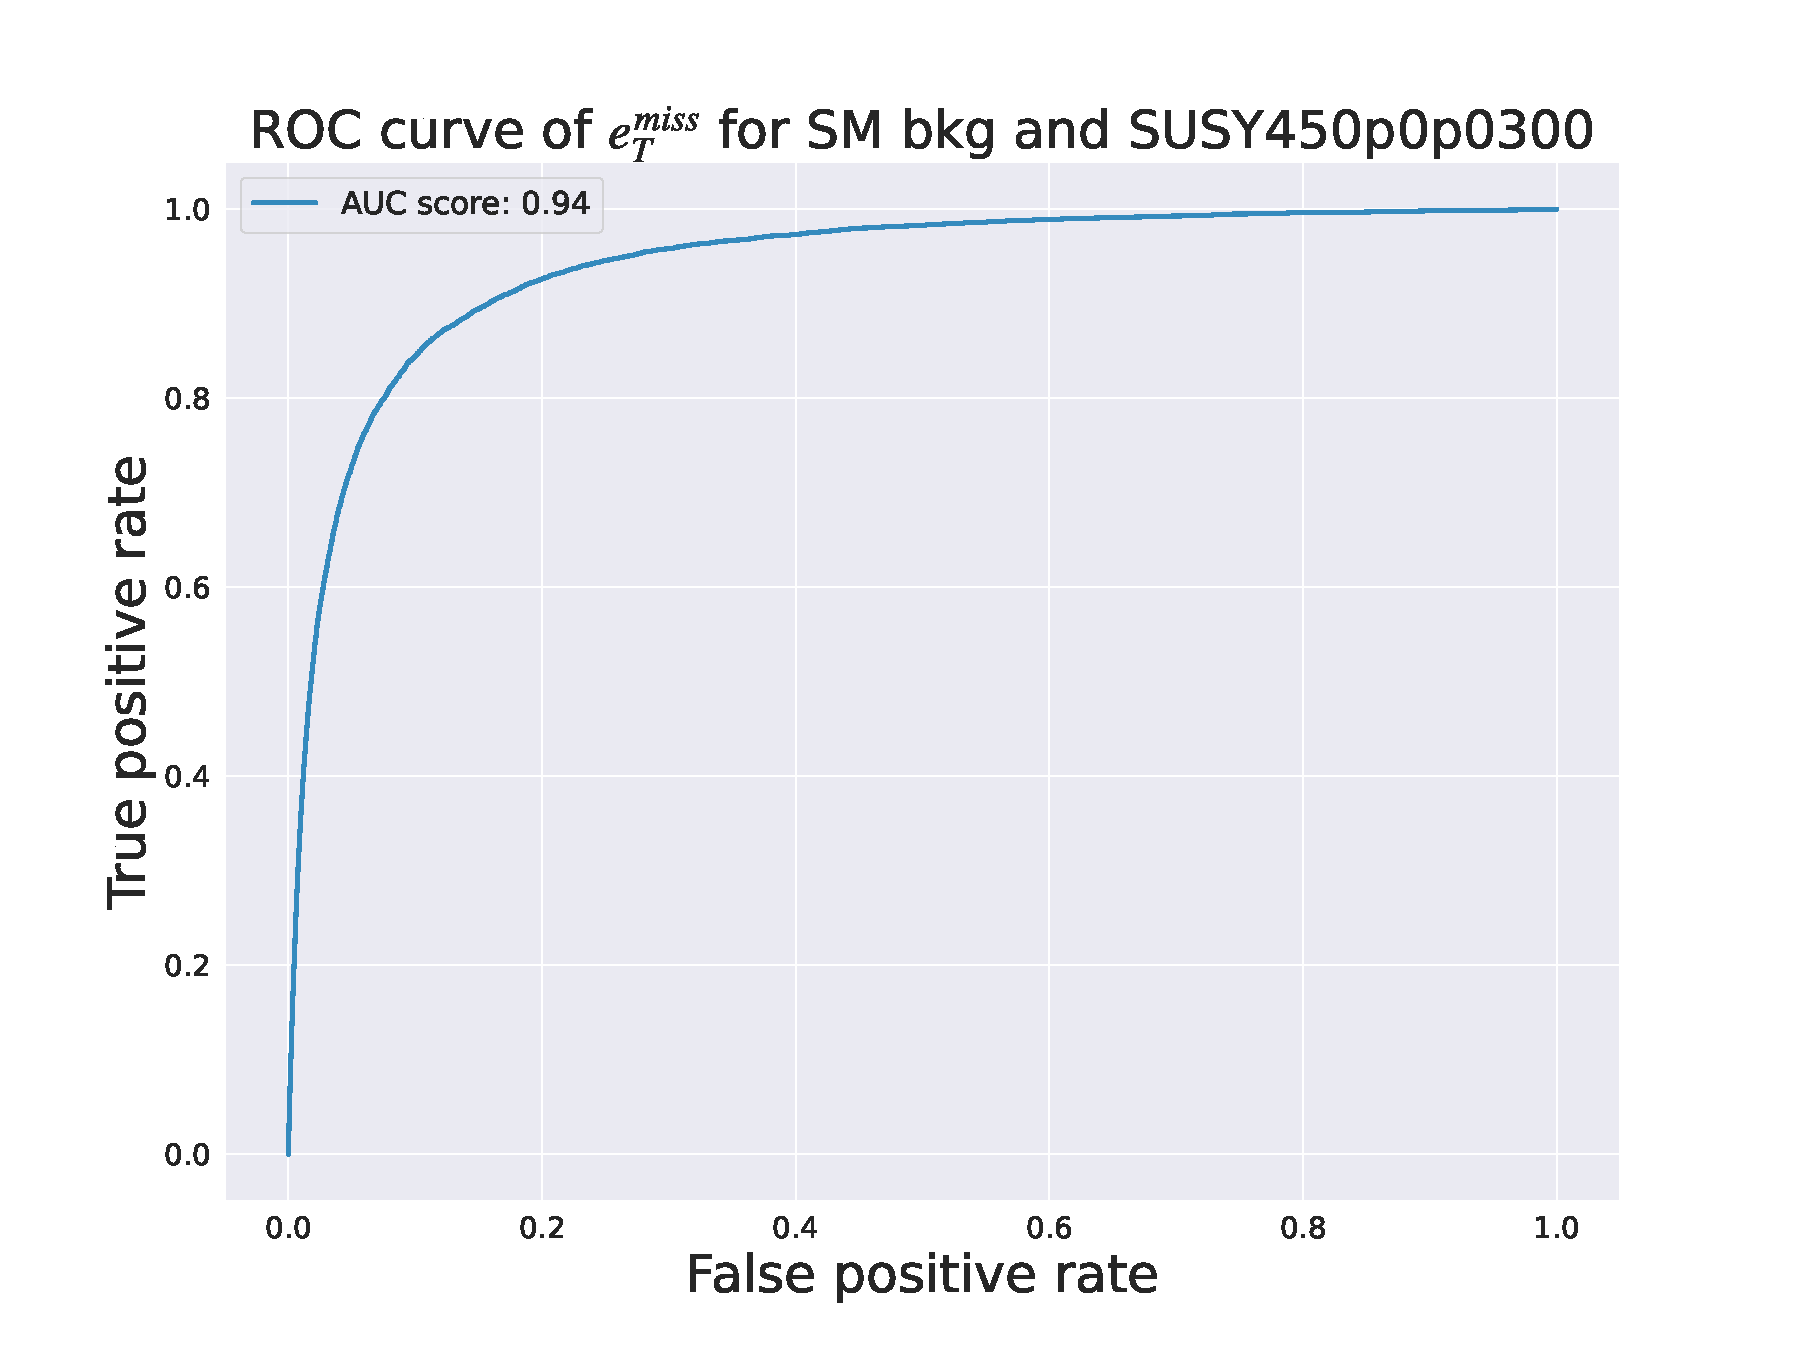
\includegraphics[width=\textwidth]{Figures/AE_testing/big/roc_curve_etmiss_450p0p0300.pdf}
        \caption{ROC curve for $e_T^{miss}$ of both SM MC and the SUSY $450-300$ signal. We see here that based on that feature alone, you can separate 
        the distributions with reative ease, with an AUC of about 0.94. }
    \end{subfigure}
    \hfill
    \begin{subfigure}{.45\textwidth}
        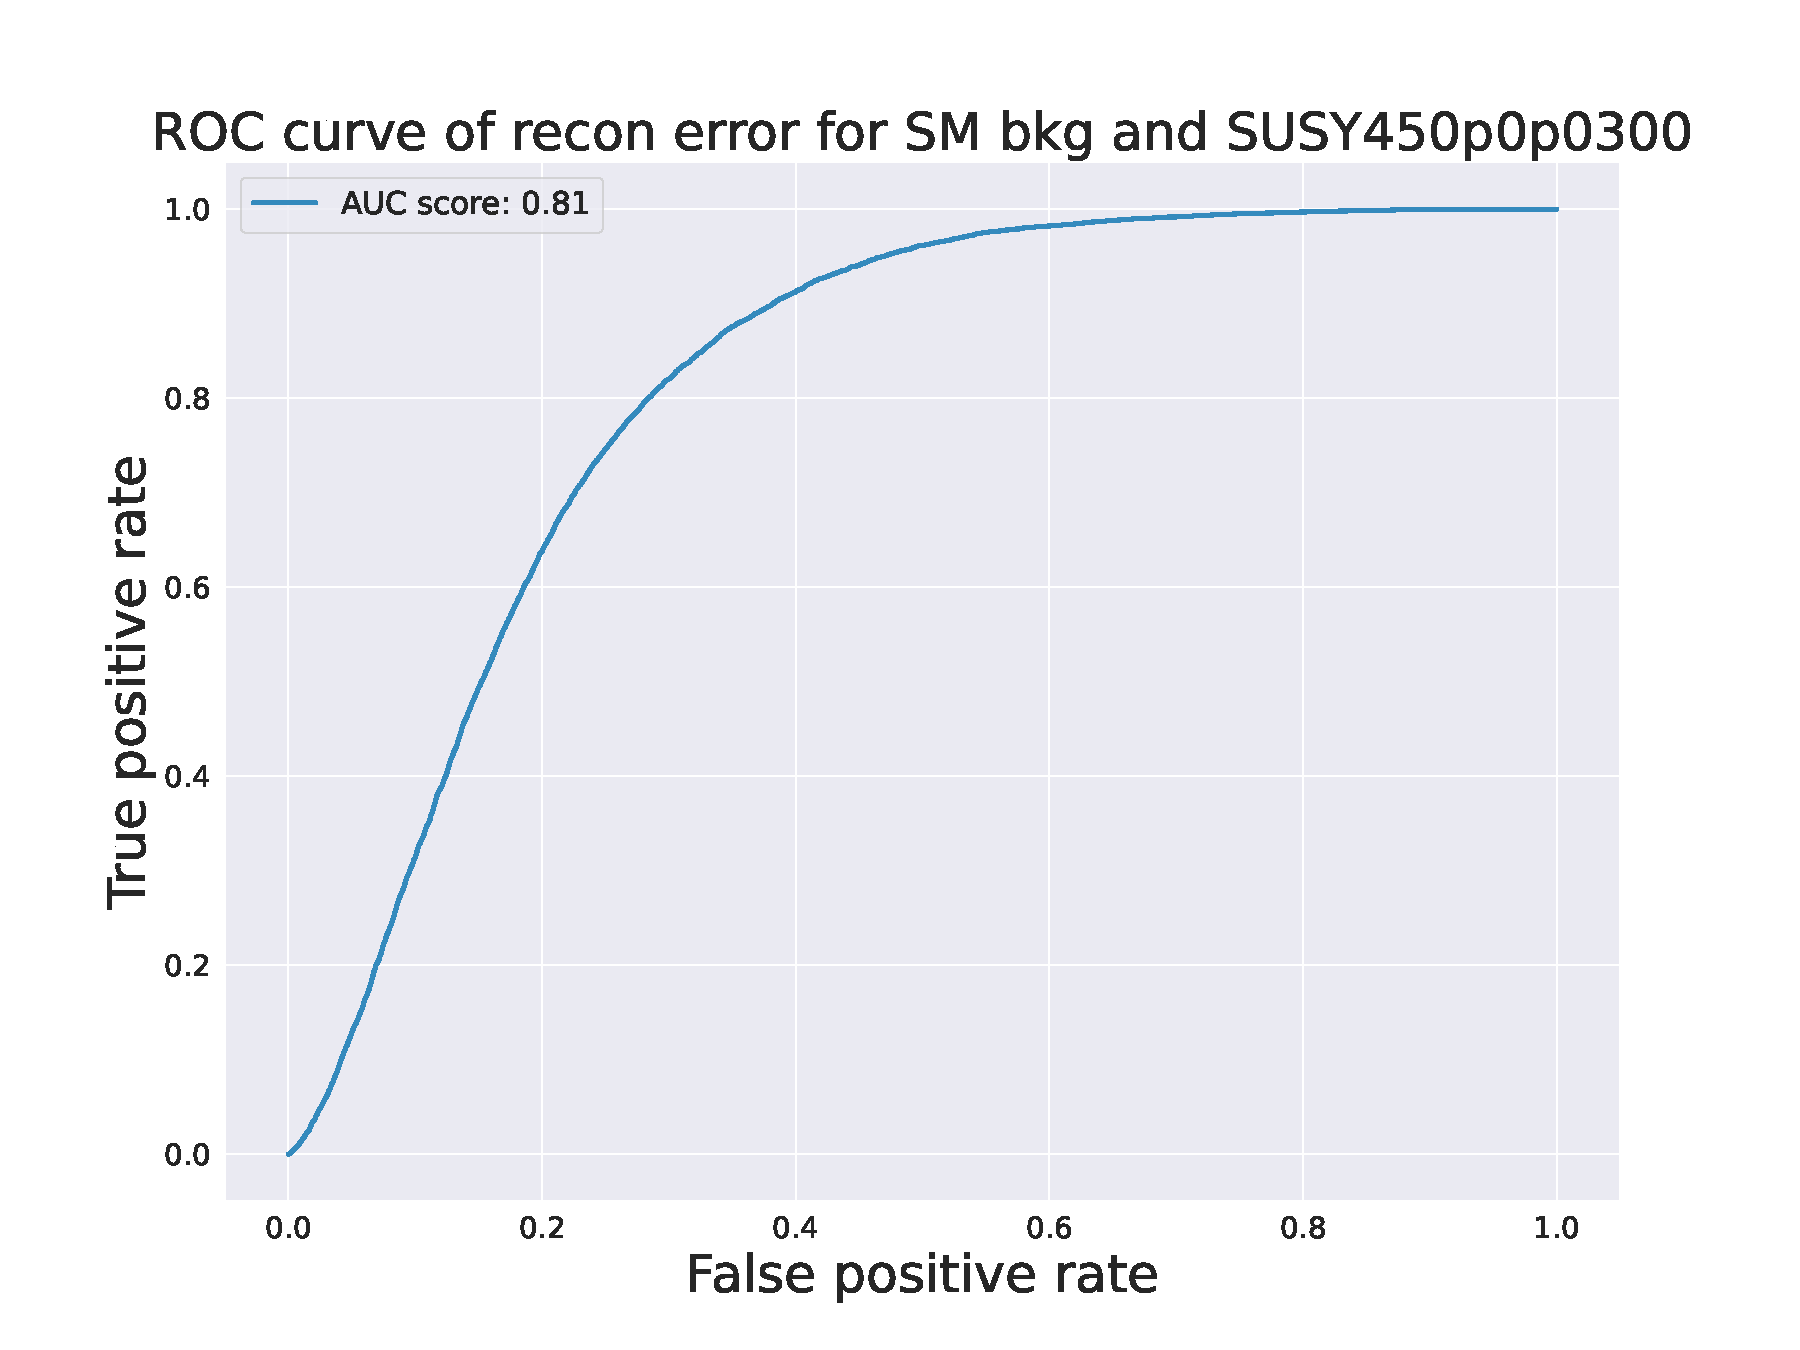
\includegraphics[width=\textwidth]{Figures/AE_testing/big/roc_curve_recon_err_450p0p0300.pdf}
            \caption{ROC curve for reconstruction error of both SM MC and the SUSY $450-300$ signal. We see here that there is relatively good separation,
            with a small AUC of about 0.81.}
        \end{subfigure}
        \hfill
    \caption{ROC curve for both $e_T^{miss}$ and reconstruction error with the SUSY $450-300$ signal. }
    \label{fig:roc_susy_450_300}
\end{figure}



\begin{figure}[h!]
    \centering
    \begin{subfigure}{.45\textwidth}
    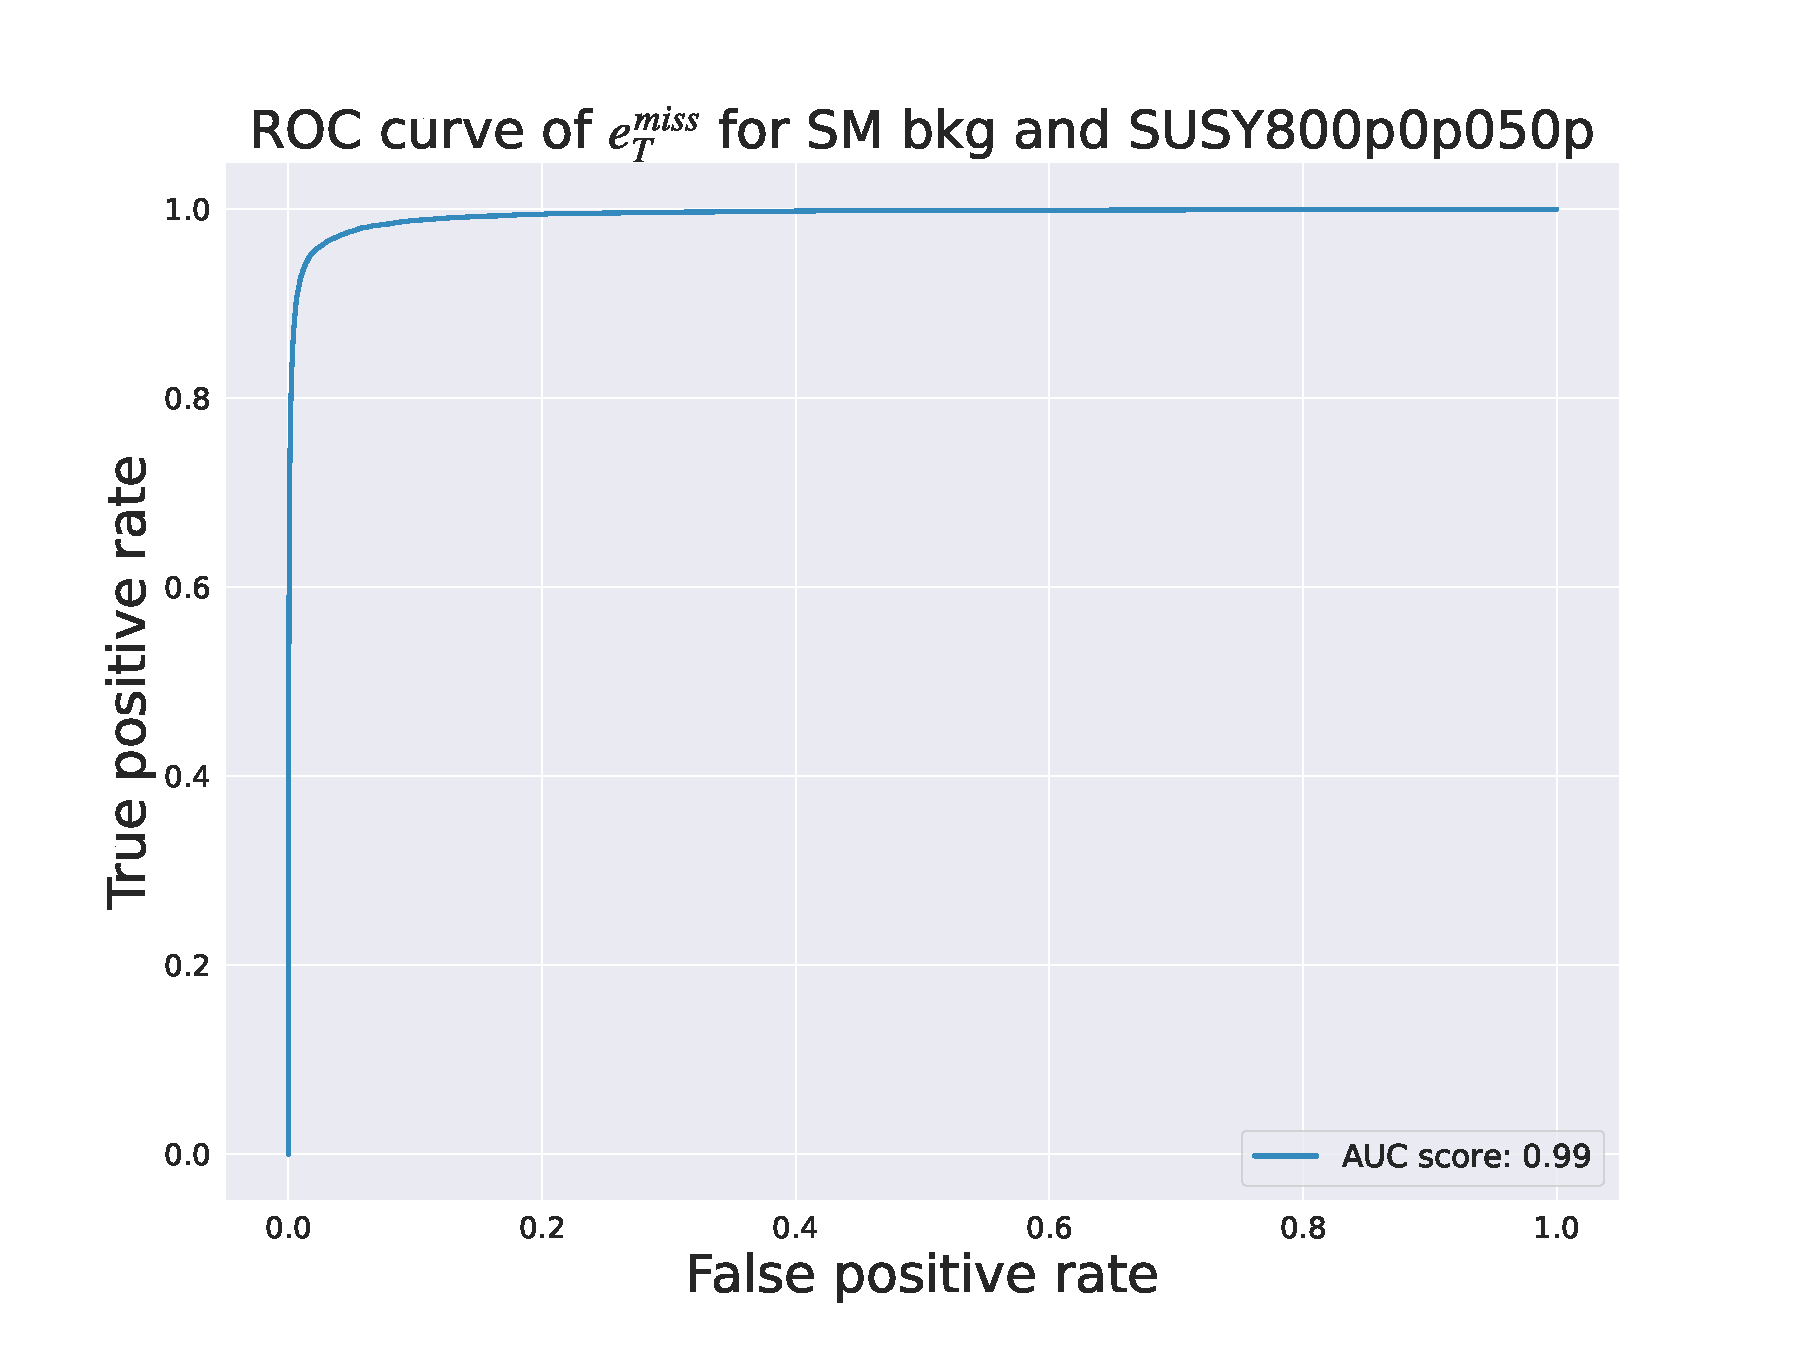
\includegraphics[width=\textwidth]{Figures/AE_testing/big/roc_curve_etmiss_800p0p050p.pdf}
        \caption{ROC curve for $e_T^{miss}$ of both SM MC and the SUSY $800-50$ signal. We see here that based on that feature alone, you can separate 
        the distributions with reative ease, with an AUC of about 0.99. }
    \end{subfigure}
    \hfill
    \begin{subfigure}{.45\textwidth}
        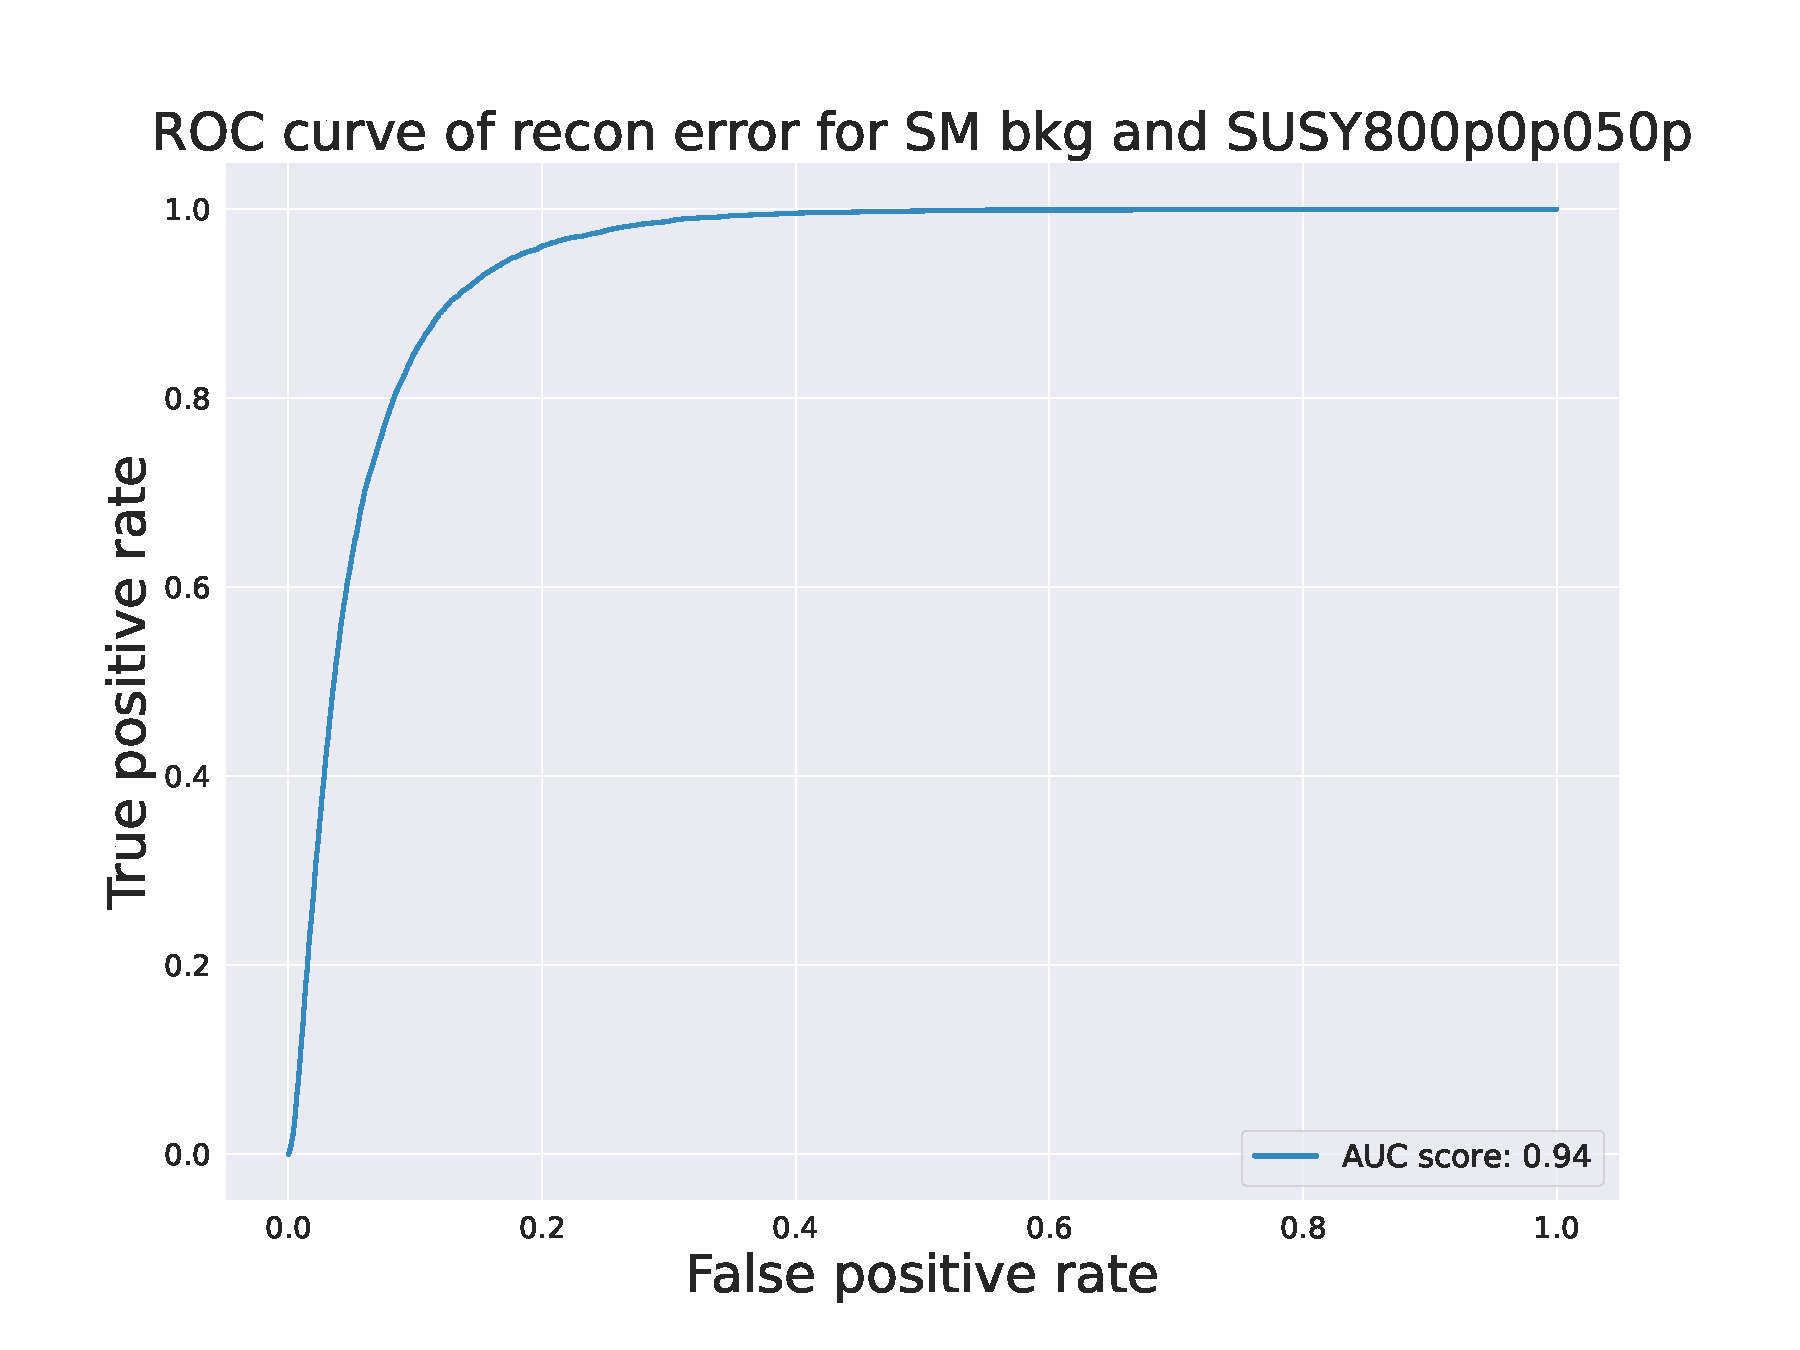
\includegraphics[width=\textwidth]{Figures/AE_testing/big/roc_curve_recon_err_800p0p050p.pdf}
            \caption{ROC curve for reconstruction error of both SM MC and the SUSY $800-50$ signal. We see here that there is a very good separation between the distributions
            , with an AUC of about 0.94.}
        \end{subfigure}
        \hfill
    \caption{ }
    \label{fig:roc_susy_800_50}
\end{figure}

From figure \ref{fig:roc_susy_450_300} and \ref{fig:roc_susy_800_50} we see that even though the reconstruction error is a good discriminator 
for the SM MC and the SUSY signals, $e_T^{miss}$ provides better separation. This is because the SUSY signals have very high $e_T^{miss}$, 
so much so that one can separate them by eye on that distribution alone. The interpretation of this is that the autoencoder has shown it 
can be used for the purpose of separating the SM MC from the SUSY signals, but not to the level of using just $e_T^{miss}$. 
The same behavior is shown for the small autoencoder in the appendix, aswell as for the small and large variational autoencoder. 